\chapter{Future Work}\label{cha:future_work}

This chapter outlines potential future directions for extending our work. Our 
thesis has investigated the connections between complex systems, open-ended 
evolution, and learning. While these fields have been studied for some time, 
many open problems still remain, some of them poorly understood, making this research exploratory
in nature. We hope that our work can advance our understanding of learning and
adaptation in natural and artificial systems, leading to the development of more
effective and efficient learning algorithms in the future.

\section{Evolving cellular automata for complexity}

The metric of complexity developed in Chapter \ref{cha:meas-compl-evolv} and the
others presented in Section \ref{sec:measuring-complexity} often gives a single
value output from a system's evolution over time. Similarly to how
\textcite{mitchellEvolvingCellularAutomata1996} evolves \acp{CA} rules to solve
a particular task, it seems appealing to use complexity as a fitness
function for a genetic algorithm. Such an algorithm would generate new rules
that are progressively more complex (according to the complexity metric).

It is difficult to apply this principle in practice. Because many complexity 
metrics such as the algorithmic complexity \ref{sec:algo-complexity} are 
approximating some uncomputable ideal value. Candidate systems that maximize a 
particular metric are often unsatisfying because they exploit a particular flaw 
of that approximation. This could be accounted for in future
work using multiple complementary complexity metrics or using another surrogate
metrics, such as the ability to learn to solve auxiliary tasks and generalize 
from basic tasks to harder ones.
This approach motivated our work in Chapter \ref{cha:learn-effic-compl}, where
we design a benchmark of progressively more complex tasks that could be used to
evaluate the ability of a system to perform complex computations.

\section{Feedback reservoir computing}

In Chapter \ref{cha:learn-effic-compl}, we explored the applications of the
\acl{RC} paradigm to \acfp{CA}. In general, \ac{RC} assumes a purely forward
model, which means that inputs are fed into the reservoir and outputs are decoded from
it. The trainable decoder layer is trained offline on a training dataset and
is then fixed during testing. We illustrate the principle of \ac{RC} in Figure
\ref{fig:classical_reservoir}. This structure is often sufficient for supervised
tasks when a sufficiently large training dataset is available.

\begin{figure}[htbp]
  \centering
  \begin{subfigure}[t]{.5\linewidth}
    \centering
    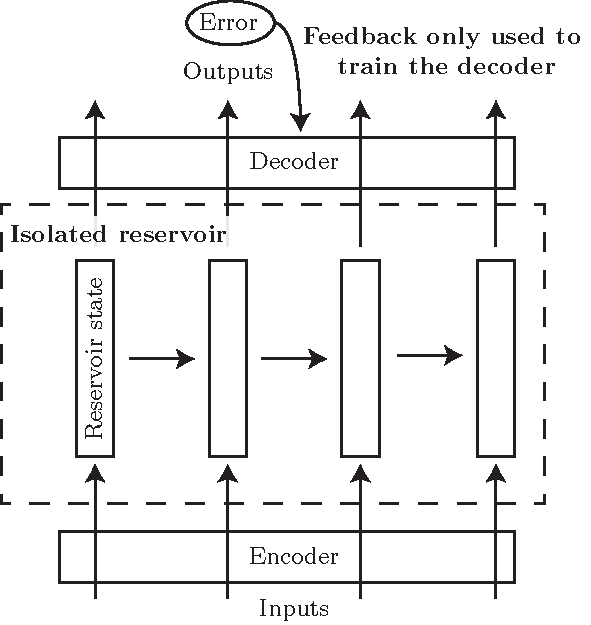
\includegraphics[width=\linewidth]{figures/classical_reservoir.pdf}
    \caption{Classical reservoir computing}
    \label{fig:classical_reservoir}
  \end{subfigure}
  \begin{subfigure}[t]{.45\linewidth}
    \centering
    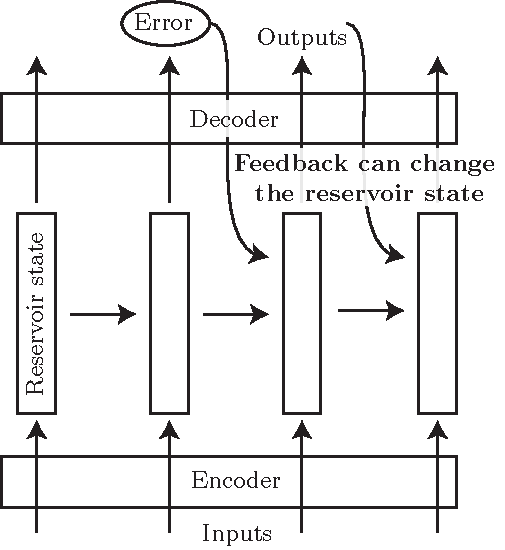
\includegraphics[width=\linewidth]{figures/feedback_reservoir.pdf}
    \caption{Feedback reservoir computing}
    \label{fig:feedback_reservoir}
  \end{subfigure}
  \caption{Comparison of regular reservoir computing with feedback reservoir
    computing. Time flows from left to right on both Figures.}
  \label{fig:reservoir_comp}
\end{figure}

A straightforward extension that could make the \ac{RC} systems fully autonomous
would be to transmit an error signal within the reservoir state at each
output. This extension we call \emph{feedback reservoir computing} is
illustrated in Figure \ref{fig:feedback_reservoir} alongside the standard
\ac{RC} model \ref{fig:classical_reservoir}. 
An ideal system would use an internal learning algorithm embedded within 
the reservoir state update function and act on the reservoir state, to 
adjust its future outputs in response to an error signal. This would enable 
the system to gradually enhance its performance over time.
The only mechanism that should be built into
this system would be an incentive to minimize the error signals received by
adaptation. The main limitation of this idea is that the design of such a system with
built-in adaptation is not easy. We do not know of a mechanism that can enable
autonomous adaptation and improvement without external input. The error signal is a 
type of external input, but it is not specified how the system should use the 
signal. Our work on
complex systems points towards cellular automata and other complex systems as
candidates for supporting such a mechanism, which would rely on the growth of
complexity.

\section{Learning in dynamical systems}

By examining the learning process in complex systems, neural networks, and
the reservoir computing framework from a unified perspective, we can
identify a generalization that provides a valuable perspective on the problem of
learning in dynamical systems. This generalization allows us to consider the
various components of these systems in a more integrated manner, enabling us to
develop a more comprehensive understanding of the underlying mechanisms of
learning without having to focus on a particular dynamical system.

This form of learning occurs dynamically as a system is simulated or run. Rather
than using traditional parameter updates, it takes place in the system's state
or ``activations'', resulting in what we refer to as \emph{learning in dynamical
  systems}. This process is analogous to an inner loop or ``thinking phase'',
during which the system can self-organize by manipulating its current state
without external changes to its parameters. This type of learning is already
present in various machine learning systems, including some \acfp{RNN}, which
use short-term dynamical learning to solve language-based tasks (see Section
\ref{sec:dynam-learn-acprnn}). Transformers are another type of neural network 
that has been popular for processing text sequences. The memory of the transformer 
is not an emergent byproduct of the training process of the neural network because 
the attention mechanism is directly processing a "window" of input tokens. Emergent 
memory is also present in some form in the \ac{RC}
framework and in the update rule of gradient-based learning algorithms. Although
effective, this form of learning is often not studied or optimized to the same
extent as more conventional methods of parameter optimization.

\paragraph{Generic model.}\label{sec:generic-model}
We give a general description of a model of learning in dynamical systems. A
dynamical system is described by a sequence of variables $S_{t}$ taking values
in some state space $\mathcal{S}$ at times indexed by $t$. In the most general setting, the
state space can be real-valued or discrete, and the time index may also be
continuous or discrete. An evolution function $f$ specifies the state of the
dynamical system at time $t$ given a history of states for $t' < t$. It may be
deterministic or stochastic.

We study the special case of discrete-time dynamical systems where the current
state depends on the previous state.

\begin{equation}
  \forall t \in \mathbb{N},\quad S_{t + 1} = f(S_{t})
  \label{eq:dyn-update}
\end{equation}

The inputs $x \in \mathcal{X}$ can be used to condition the update rule and enable the dynamical system
to interact with an environment. The space $\mathcal{X}$ can be chosen arbitrarily, 
for example, the space of real vectors in dimension $n$, $\mathcal{X} = \mathbb{R}^n$. 
For an input $x$, we can write the new dynamical update equation

\begin{equation}
S_{t+1} = f(S_t, x).
\label{eq:11}
\end{equation}

Outputs can be observed from the current state $S_t$ with a decoding function
$D$. We define the output for time step $t$,
\begin{equation}
  \label{eq:10}
  y_t = D(S_t).
\end{equation}
Depending on the use cases, alternate representations may be considered where
the output depends on two or more time steps or an input vector $x$.
We give a few well-known examples of learning in dynamical systems from the
field of machine learning.

\paragraph{Dynamical learning in \acp{RNN}}\label{sec:dynam-learn-acprnn}
We study the example of a question-answering task with a pre-trained \ac{RNN}.
It is easy to see that a \ac{RNN} can be written fully using \eqref{eq:11} and
\eqref{eq:10}. The task of answering questions is about reading information from
a prompt and answering a question that involves recalling some data from the
prompt. An example of such a prompt and question:
\begin{equation*}
  \underbrace{\texttt{Two cats and five dogs sleep on the red mat.}}_{\text{Prompt}}
  \underbrace{\texttt{How many dogs are there?}}_{\text{Question}}
\end{equation*}
More advanced question answering requires reasoning and advanced processing of
the prompt. In the above example, it would suffice to remember the words of the
prompt.

We consider a trained \ac{RNN} evaluated on a set of question-answering tests.
If the data set was designed correctly, the network should not have prior
information about a sentence/question pair before reading it. The relevant piece
of information of the prompt has to be stored within the values of the hidden
state of the \ac{RNN} and not in the weights of the neural network since they are not changed during this phase. This transient learning that enables the
\ac{RNN} to memorize the beginning of the prompt is exactly the type of
dynamical learning that we describe above. \acp{RNN} are trained offline to
achieve this, but once they are trained, learning happens dynamically.

Modern \acp{RNN} are not designed to take full advantage of this memory
property and will progressively overwrite the memory if run for more timesteps.
Still, they illustrate the type of learning we want to emphasize. We expect
advanced systems to be able to keep that memory and also be capable of
manipulating stored information to construct a reasoning and form novel concepts.

\paragraph{Supervised learning with stochastic gradient descent.}
\label{sec:superv-learn-with}
We consider another example: a single hidden layer neural network with weight
matrices $W_1 \in \mathbb{R}^{n \times d}$ and $W_2 \in \mathbb{R}^{d \times o}$. We train the network with
standard backpropagation and stochastic gradient descent with a learning rate $\tau$.
The neural network is represented by a function $F$, and the loss function
between the network output and the label is written as $\mathcal{L}$.

Using the notation of Section \ref{sec:generic-model}, we define
$S_{t} = \left(W_{1}^{(t)}, W_{2}^{(t)}\right) \in \mathbb{R}^{n \times d} \times \mathbb{R}^{d \times o}$
containing the neural network parameters at step $t$ of the training. We assume
that the training pairs $(X_{k}, y_{k})$ are numbered according to their
selection order for the stochastic gradient descent algorithm.
The stochastic gradient update function for the state $S_{t}$ is:
\begin{equation}
  \label{eq:supervised-learning}
  S_{t+1} = {f}(S_t, X_t, y_t) = \left(W_1^{(t)} - \tau \frac{\partial
      \mathcal{L}(F(X_t), y_t)}{\partial W_1^{(t)}}, W_2^{(t)} - \tau \frac{\partial
      \mathcal{L}(F(X_t), y_t)}{\partial W_2^{(t)}} \right).
\end{equation}

Note that the function $f$ is deterministic for a given ordering of training
pairs. Therefore, the stochasticity of $f$ is contained in the numbering of
training examples.

\begin{figure}[htbp]
  \centering
  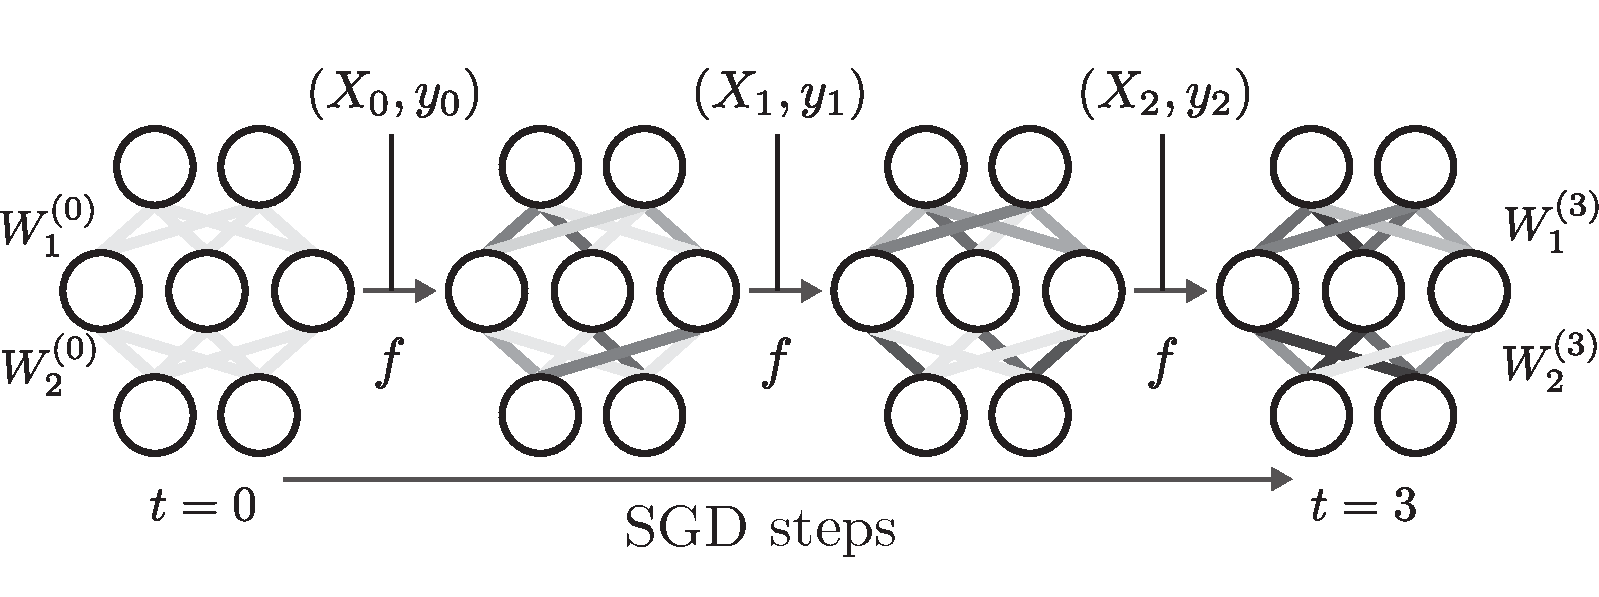
\includegraphics[width=.9\linewidth]{figures/learning_nn.pdf}
  \caption{\label{fig:label} Learning happens within the ``activations'' of this
    dynamical system, which in this example are the weights of a neural
    network being updated with the stochastic gradient descent algorithm (SGD). 
    The fixed update function depends on an input pair $(X, y)$
    and the previous state vector $S = (W_1, W_2)$.}
\end{figure}

We note that $f$ is a fixed update function (from the dynamical system point of
view of the training pipeline, a training input/output pair $(X, y)$ is a pair
of input values). In supervised learning, the function $f$ causes the state to
converge to a fixed point. This property is desired when solving a target task
characterized by a loss $\mathcal{L}$. Because of that convergence property, a neural
network cannot be expected to produce any novel behavior after the end of its
training. On the contrary, we know that other complex dynamical systems that we
study in this thesis, like cellular automata, may exhibit a behavior of increasing
complexity during their development, with no sign of convergence towards a
stable state.
